% !TeX root = ../main.tex
% Add the above to each chapter to make compiling the PDF easier in some editors.

\chapter{Introduction}\label{chapter:introduction}

\section{Background}
\label{background}
Internet of Things (IoT) has become an emerging technology with the power of low priced computational units and the cloud technology. There are thousands of different examples in the real world which targets both the end-users and the industry. 

The problem with the current state of the art is the requirement of tremendous time investment by the developers. The developers need to spend this time to develop both embedded software and web services to serve their goal. The most of this time is spent on functionalities that are already implemented in different projects with slight differences.

In IoT practical course offered in the Technical University of Munich, the hardware abstraction layer for single board computers is built. This layer has been extended to a platform with IoT core which covers required web services functionalities to store and access the data of the devices with multi-protocol support. In the following semesters, the development of this platform will be sustained. The goal of this platform is to solve the challenges and problems of the developers concerning need of technical background and time by serving a configurable platform with an easy-to-use user interface. This generic and practical platform can be extended with the easily configurable rule engine to process live data streams or historical data batches of the devices.

In most cases, the applications have similar capability needs to process their data with some little customization. The most basic needs during the data process flow can be listed as;
\begin{itemize}
  \item Retrieving the data,
  \item Checking whether a data point in a data stream satisfies a condition,
  \item Checking whether a data batch in historical data satisfies a condition,
  \item Forwarding the data to another data process flow,
  \item Manipulating the data,
  \item Classifying the data,
  \item Triggering defined events.
\end{itemize}

There are various challenges while achieving systems which are capable of operating the requirements above. Availability, the need of time, integration of a new process into the system and the vast number of different devices can be considered as these challenges.

The required functionalities to define data process flows in the area of IoT diverge from each other with only a little customization. Business logic, interoperability of the sensors and actuators, machine to machine (M2M) communication and context-aware services are the divergency items and the primary concern for each IoT systems \cite{6651222}. Therefore, any abstraction to define functionalities shall also allow fundamental freedom not to lose these divergency items.

To point out the challenges in the current state of the art within an example, a corporate company which delivers IoT solutions for the factory automation systems can be taken into account. This corporate company customizes their system to match with the needs of their customers. In the scope of data processing, this customization may be adding the support of the different type of devices, introducing new methods into the data flow, implementation of brand-new feature or integration of features that are already implemented in the past for another customer.

All of these customizations may lead to challenges which will end up with hiring new developers or losing the potential customers. A generic and practical rule engine can be defined to implement and to maintain the functionalities of the necessary system in the IoT domain. The predefined and parameterized building blocks within a functional user interface (UI) and application program interface (API) can sustain a fast and practical environment to ease and erase these challenges.

\section{Proposed Solution}

This master thesis aims to build an ontology-based rule engine to define data flows needed for web services in the area of IoT within a generic and practical development environment. An abstraction of all functionalities that are necessary for any data flow would help to achieve this generic rule engine. The predefined and customizable building blocks, ontologies to store the data and the rules are crucial for a generic and practical platform with the help of the abstraction. On the other hand, the genericity would be a challenge to accomplish the practicality goal. So to maintain practicality, the resulting platform shall be definite and comprehensive enough to support any IoT project and the other areas shall not be a concern. In other words, the building blocks shall not be too broad to support any domain. Additionally, all customization concerning each building blocks shall be done in easy-to-use interfaces that are supplied to the users to maintain practicality. 

While designing web services that will be used in different use cases in IoT as well as others, some design concerns must be taken into account by the developers. The techniques and the architecture to enable communication between all necessary nodes, the format for the data that will be stored, how and when data will be served can be considered as the primary design concerns \cite{6651222}. After the design phase of the system has been finished, the design shall be easily implemented to make the prototypes live and to run them. 

The resulting platform will provide solutions in different degrees for the practicality challenges and problems in the IoT domain. These challenges and issues can be listed as follows;

\begin{enumerate}
    \item The requirement of the technical background,
    \item The need for the time investment,
    \item The maintenance of the system,
    \item The reimplementation of already implemented functionality,
    \item The deployment of the system,
    \item The different technology backgrounds of the developer in the team.
\end{enumerate}

There exist different options with different practicality levels to implement the designed web services in the platform. 

The platform that is based on the rule engine provides the solutions to the developers to solve the problem of the requirement of an enormous amount of time investment and technical background, and maintenance challenge by simplifying the working environment. The platform shall render a practical and easy to learn web UI for the hobby users with a less technical background. The data and the rules, which are owned by the platform user, will be easily accessible and mutable by the platform user in the UI. The platform users will quickly adapt even if they have little technical background since the system provides building blocks to connect with each other by using the most common user experience (UX) elements such as drag-drop objects, wires, and forms. 

The platform shall also store the data of the web applications of the platform users in an easily accessible, organizable and modifiable way without loss of genericity. M. G. Kibria et al. proposed that a semantic ontology which declares every device as objects on the gateways can be used for the energy efficiency \cite{7993747}. N. Lee and H. Lee also suggested an IoT service architecture that provides services with an object gateway \cite{6884496}. The device objectification by using ontologies is a reliable method to store the data of the real world devices in IoT services. Nevertheless, the management of read-write access to the objects, the evaluation of the gathered data and the methods for the service of these data are the topics that need to be covered to build a generic and practical platform that serves any needs of IoT.

To build business logic and define evaluation methods on the ontologies; the rules, which are in if-then form decision-making tools, must be introduced in the platform. The rules function like a chain of blocks, where each does a small fraction of the functionality while interpreting the logic.  There are different types of blocks that each has a different function in the rule handling. The limited toolbox of generic rule blocks also preserves the practicality for the users since they do not need to master a vast pool of different block types.

In addition to these simplifications, the platform also supports reusability of any functionality or data hierarchy to avoid reimplementation challenge. Therefore, the developers such as in the corporate company that is given in the subsection \ref{background} will not need to reimplement functionalities that are required a new customer. Instead, they will reference the data or the features that are already implemented for another customer.


The deployment of the system will be easier for the most basic user with the existing UI. However, there will be more tools for the power users to handle their deployment challenge. The power users such as working in a corporate company are provided with application program interface (API) to use any functionality of the platform through HTTP requests and Internet of Things Easy Query Language (IoTeQL) to manipulate their data and rules as well as the UI for their basic operations on their system. With the help of API and IoTeQL, existing systems such as the system of the corporate company can be transferred to the platform quickly with the help of a script. Moreover, when the corporate company needs to provide their services with a little customization for a new customer, they can quickly achieve it by using reusable components.

Since the platform is technology independent and focuses on the construction of the logic, different technology background of the team members will not be a concern for the developer teams. They will easily adapt to the development environment of the platform with any background.
\clearpage
\begin{figure}[h]
  \centering
  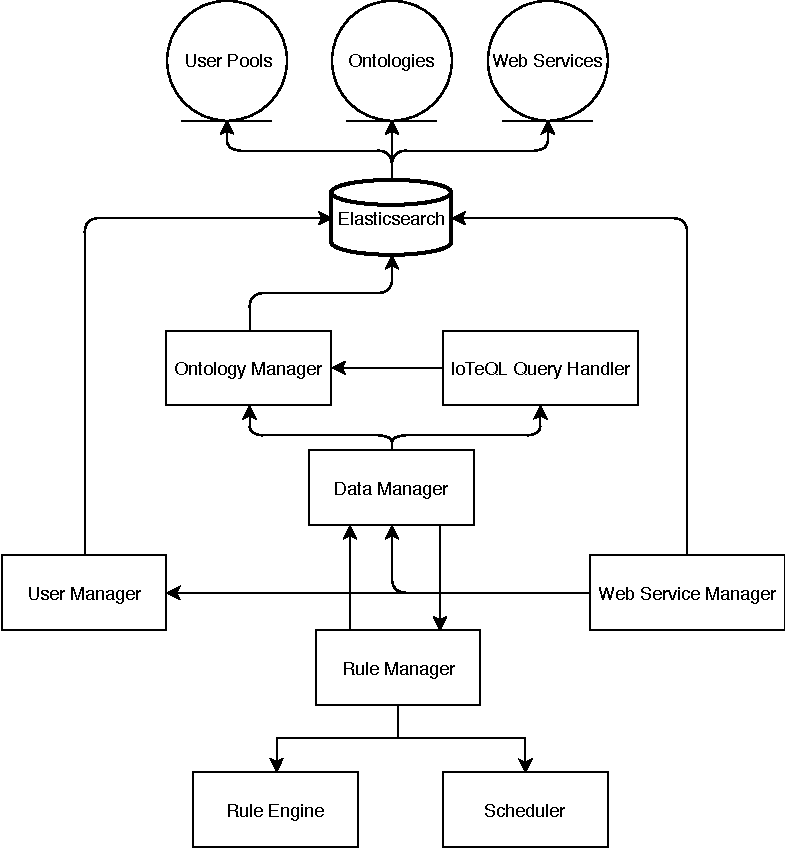
\includegraphics[width=0.4\textwidth,height=\textheight,keepaspectratio]{figures/high_level_architectural_diagram.pdf}
  \caption[Platform Architecture]{The high level architectural diagram of the platform}\label{fig:architecture}
\end{figure}

In figure \ref{fig:architecture}, the high-level architecture of the rule manager and the helper components is shown. The rule manager is tasked with running any rule when they are intended on the data. The management of the data and the rules on the ontology is the responsibility of the data manager. Since they are isolated and loosely coupled with each other, they can autoscale individually behind a load balancer and expansion of the computational unit where it is needed can be achieved. Consequently, only the data manager will horizontally scale when the number of queries is increased, or just the rule manager will scale horizontally when the massive amount of scheduled rules is needed to be handled at the same time. A platform user can access all of the subsystems by their APIs, and the connector components of them act like adapter to interact with each other. Therefore, any change in any subsystem will not lead change in overall architecture.
